
	\begin{figure}[htbp]
		\centering
		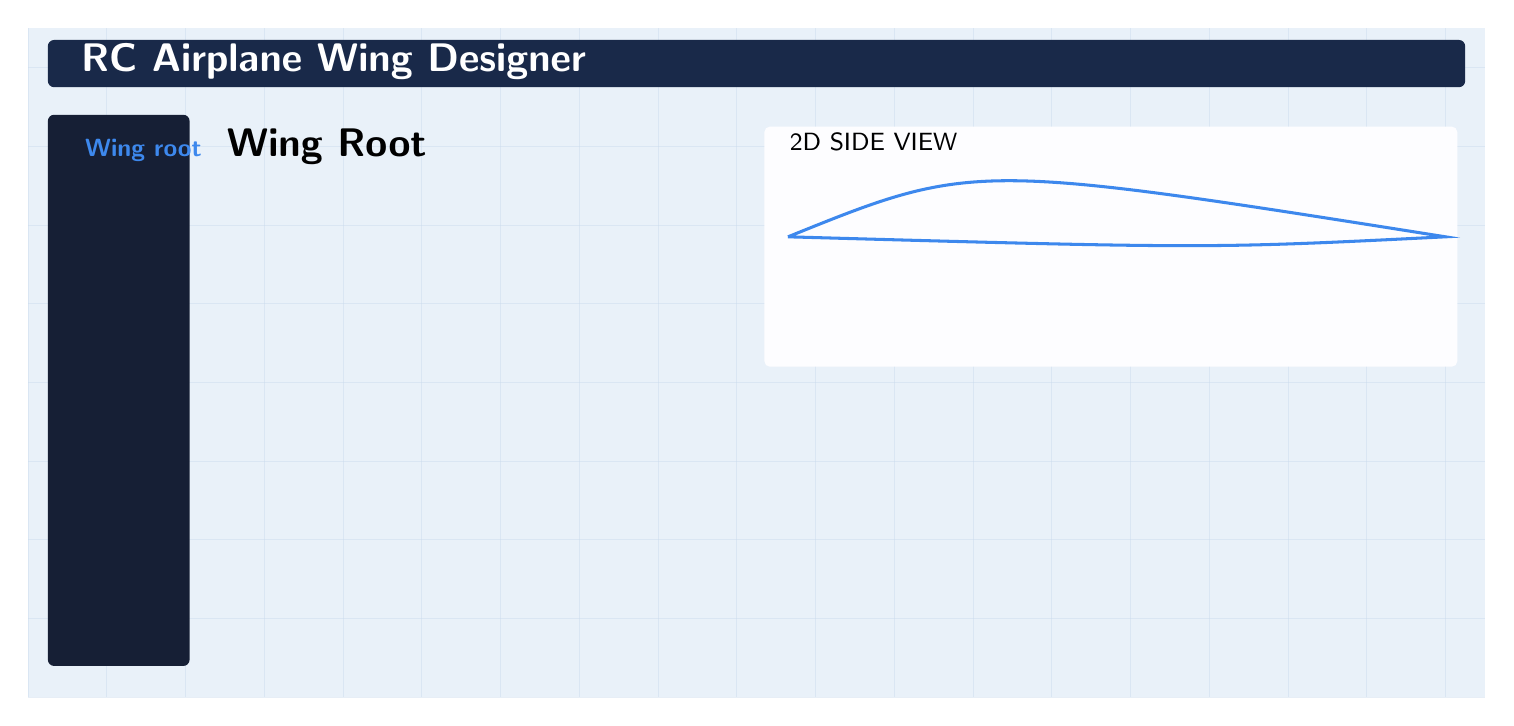
\begin{tikzpicture}[x=1cm,y=1cm]
			
			% UI-Design-Farben
			\definecolor{bg}{RGB}{233,241,249}
			\definecolor{grid}{RGB}{201,218,236}
			\definecolor{header}{RGB}{25,41,73}
			\definecolor{sidebar}{RGB}{22,31,53}
			\definecolor{accent}{RGB}{61,136,237}
			\definecolor{panelbg}{RGB}{253,253,255}
			
			% Hintergrund & Grid
			\fill[bg] (0,0) rectangle (18.5,8.5);
			\foreach \x in {0,1,...,18} {\draw[grid, line width=0.35pt, opacity=0.45] (\x,0) -- (\x,8.5);}
			\foreach \y in {0,1,...,8} {\draw[grid, line width=0.35pt, opacity=0.45] (0,\y) -- (18.5,\y);}
			
			% Header
			\fill[header, rounded corners=0.08cm] (0.25,7.75) rectangle (18.25,8.35);
			\node[anchor=west, text=white, font=\sffamily\bfseries\Large] at (0.55,8.08) {RC Airplane Wing Designer};
			
			% Sidebar
			\fill[sidebar, rounded corners=0.08cm] (0.25,0.4) rectangle (2.05,7.4);
			\node[anchor=west, text=accent, font=\sffamily\small\bfseries] at (0.6,6.95) {Wing root};
			
			% Content Bereich
			\node[anchor=west, font=\sffamily\bfseries\Large] at (2.4,7.0) {Wing Root};
			\fill[panelbg, rounded corners=0.07cm] (9.35,4.2) rectangle (18.15,7.25);
			\node[anchor=west, font=\sffamily\small] at (9.55,7.05) {2D SIDE VIEW};
			
			% Flügelprofil-Skizze
			\draw[accent, line width=1.1pt] (9.65,5.85) .. controls (12,6.8) .. (18,5.85) .. controls (15,5.7) .. (9.65,5.85);
			
		\end{tikzpicture}
		\caption{UI-Nachbau für dein Dokument}
	\end{figure}
	
\end{document}